\chapter{Triển khai của hệ thống Storm SmartHome}

Trong chương này, đồ án sẽ trình bảy triển khai hệ thống xử lý dữ liệu SmartHome xây dựng trên nền tảng Apache Storm trong hai loại môi trường huấn luyện và đánh giá. Tiếp đó là triển khai các chương trình dự đoán tài nguyên và tự động co dãn các máy ảo đa cấp độ trên môi trường điện toán đám mây. Hệ thống được triển khai tại đây sẽ làm cơ sở để đánh giá hiệu quả hệ thống trong và đưa ra kết luận trong các chương tiếp theo.

Trong cả hai giai đoạn đánh giá và huấn luyện đều có cùng các thành phần giống nhau, nội dung chính được trình bày sau đây sẽ đi vào mô tả chi tiết quá trình triển khai và thiết lập của từng thành phần.

\paragraph{Hệ thống tạo dữ liệu của Storm SmartHome}

MQTT publisher được triển khai trên cùng máy chủ với các thành phần của cụm Storm hoặc được triển khai thành máy ảo riêng biệt trong giai đoạn đánh giá. MQTT broker được sử dụng sẽ là broker công cộng EMQX: \href{broker.emqx.io}. Sử dụng broker công cộng sẽ giúp hệ thống mô phỏng tương tác giống với môi trường thực tế hơn khi có độ trễ giữa các gói tin được truyền đi.

Tại thư mục mqtt của bộ nguồn của đồ án \autocite{lemionday_thesis_storm} bao gồm một tệp docker-compose.yml và hai tệp thực thi publish-training.sh và publish-evaluate.sh. Trong đó tệp docker-compose.yml sẽ định nghĩa 6 dịch vụ tương ứng với nguồn phát dữ liệu iot của 6 tòa nhà từ 0 đến 5, tốc độ truyền tin của tất cả các tòa nhà đều được thiết lập là giới hạn 30 gói tin/giấy. Hai tệp thực thi còn lại sẽ định nghĩa các tập dòng lệnh triển khai tương ứng với giai đoạn huấn luyện và đánh giá. Khoảng thời gian giữa mỗi lần thực hiện dòng lệnh là 10 phút nhằm mô phỏng một cách ngẫu nhiên lưu lượng các gói tin thay đổi theo thời gian.

\begin{figure}[H]
    \centering
    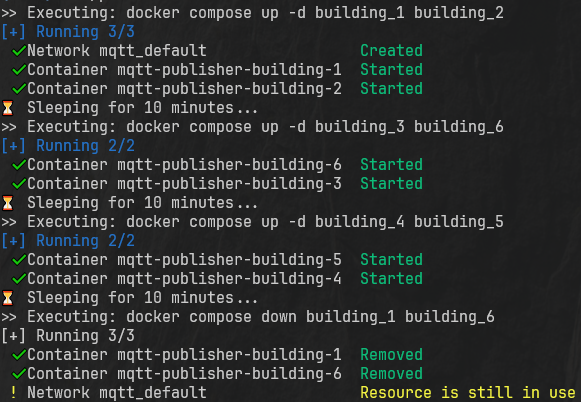
\includegraphics[width=\textwidth]{training-publish.png}
    \caption{Thực thi tệp mô phỏng gửi dữ liệu}
\end{figure}

\section{Hệ thống theo dõi, đánh giá, trực quan hóa dữ liệu}

\paragraph{Storm UI}

Triển khai Storm UI để cung cấp API cho phép Storm exporter thu thập các chỉ số.

\begin{figure}[H]
    \centering
    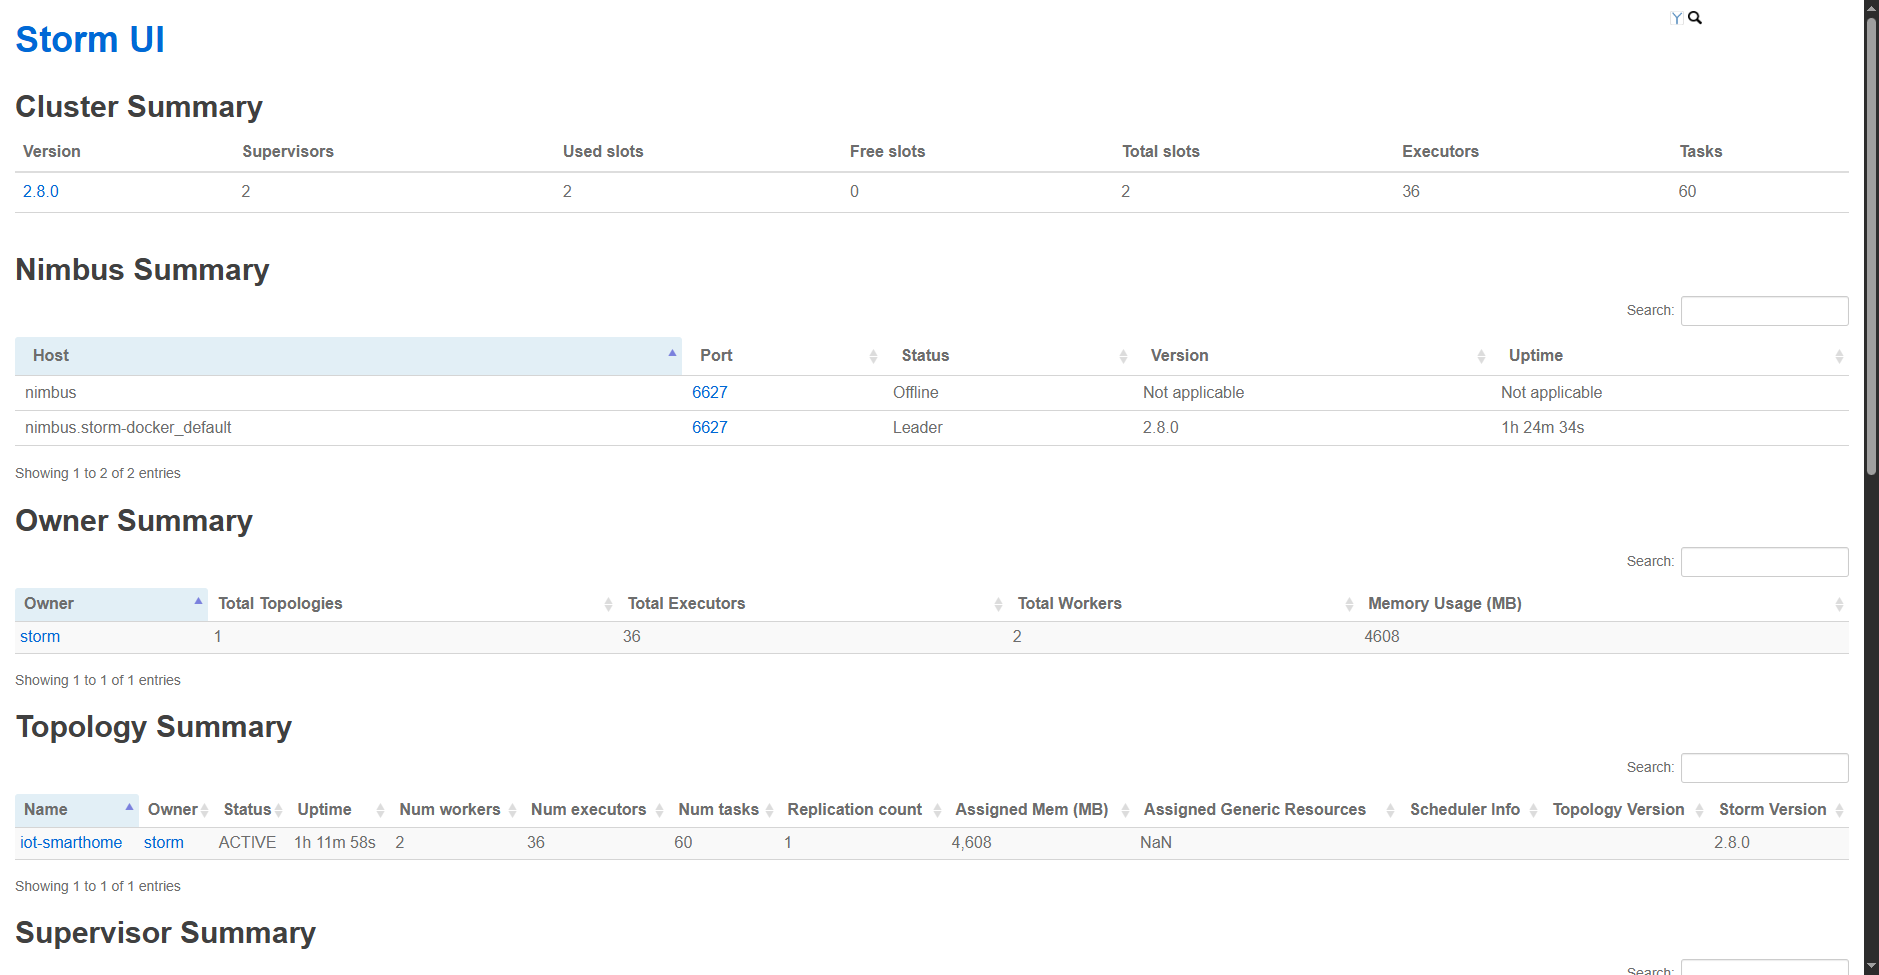
\includegraphics[width=\textwidth]{storm-ui.png}
    \caption{Storm UI}
\end{figure}

\paragraph{Storm Exporter}

Triển khai Storm exporter trên cùng tệp docker compose với storm-ui để thu thập các chỉ số từ topology và supervisor, sử dụng kèm với image socket-proxy \autocite{linuxserver_socket-proxy} để expose Docker socket làm phương tiện giúp Storm exporter đọc dữ liệu trong môi trường huấn luyện thông qua Docker API.

\begin{lstlisting}[language=yaml, caption={Cấu hình triển khai Storm exporter}]
services:
  socket-proxy:
    image: lscr.io/linuxserver/socket-proxy:latest
    container_name: socket-proxy
    environment:
      - CONTAINERS=1
      - EVENTS=1
      - PING=1
      - VERSION=1
    volumes: [/var/run/docker.sock:/var/run/docker.sock:ro]
    restart: unless-stopped
    read_only: true
    tmpfs: [/run]

  storm-exporter:
    build:
      context: .
    container_name: storm-exporter
    restart: always
    environment:
      - STORM_UI_HOST=${STORM_UI_HOST}:${STORM_UI_PORT}
      - REFRESH_INTERVAL=${STORM_EXPORTER_REFRESH_INTERVAL}
      - EXPORTER_LISTEN_ADDR=:${STORM_EXPORTER_PORT}
      - DOCKER_HOST=tcp://socket-proxy:2375
    ports: ['${STORM_EXPORTER_PORT}:${STORM_EXPORTER_PORT}']
    depends_on: [socket-proxy]
\end{lstlisting}

\paragraph{Grafana}
Grafana được triển khai trên máy chủ nội bộ trong cả hai giai đoạn.

\begin{center}
    \begin{figure}[H]
        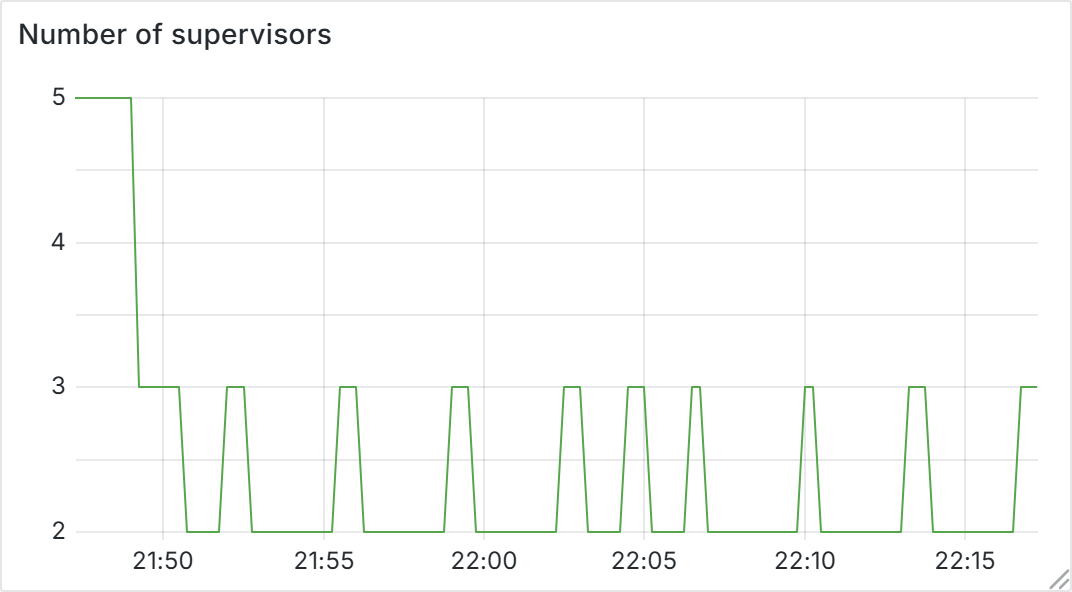
\includegraphics[width=\textwidth]{grafana-number-of-supervisor.png}
        \caption{Theo dõi số lượng supervisor của cụm Apache Storm}
    \end{figure}

    \begin{figure}[H]
        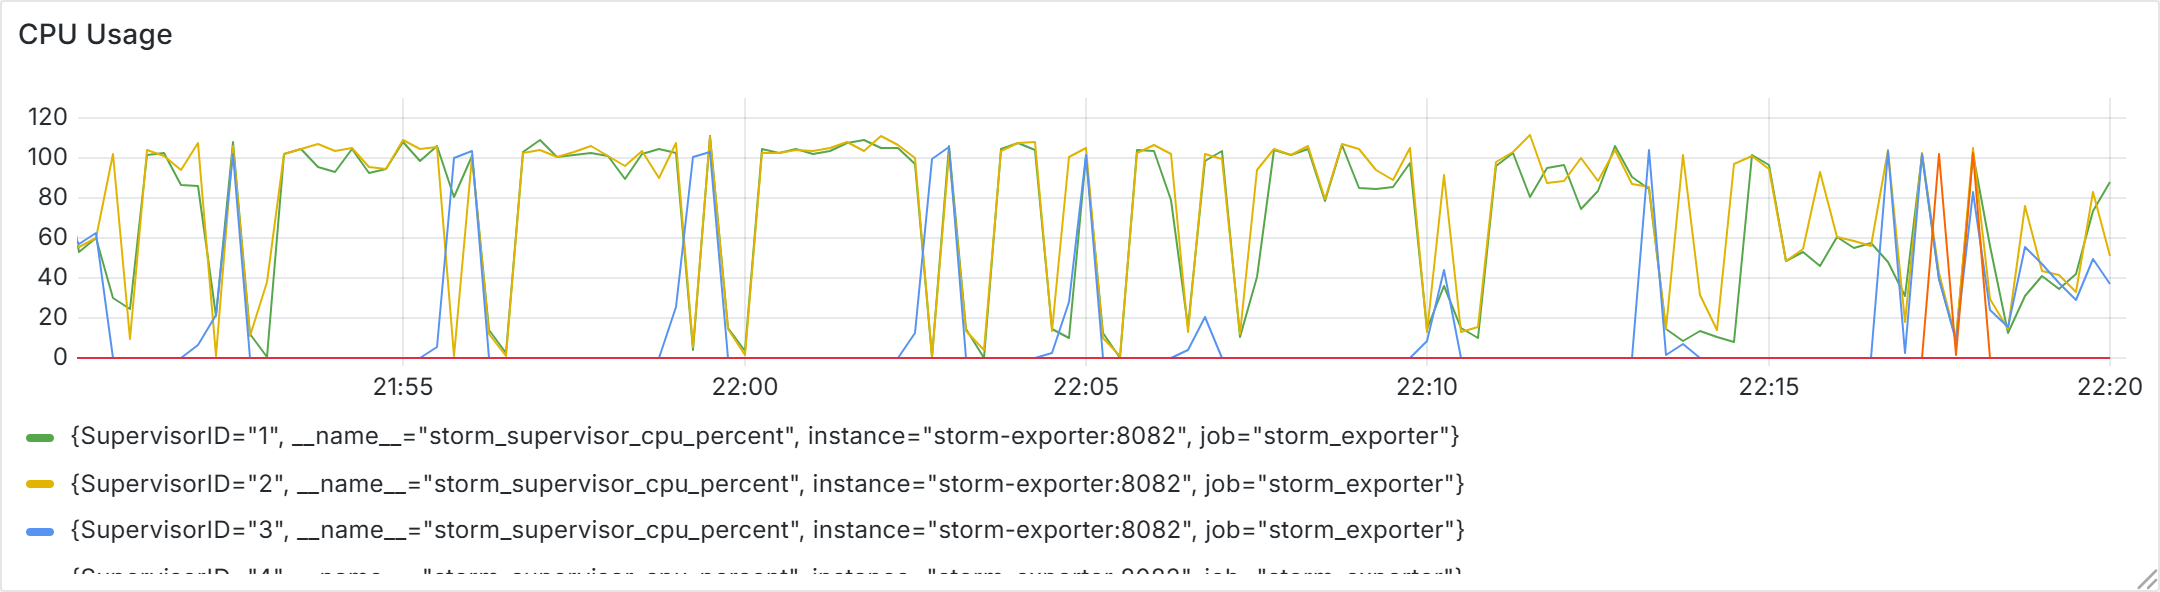
\includegraphics[width=\textwidth]{grafana-cpu-usage.png}
        \caption{Theo dõi tỷ lệ sử dụng CPU của từng supervisor}
    \end{figure}
\end{center}

\section{Hệ thống dự đoán tài nguyên và co/dãn}

Chương trình co/dãn tài nguyên được tác giả viết và lưu trữ trong thư mục autoscaler tại bộ mã nguồn của đồ án \autocite{lemionday_thesis_storm}. Để khởi chạy chương trình, có hai phương pháp

\begin{itemize}
    \item Build và chạy chương trình tại cùng máy chủ với Storm nimbus. Khả dụng cho cả giai đoạn huấn luyện lẫn đánh giá. Lệnh chạy:
          \begin{verbatim}
go build -o build/storm-autoscaler
ENVIRONMENT=Docker build/storm-autoscaler # môi trường huấn luyện
ENVIRONMENT=GCP build/storm-autoscaler # môi trường đánh giá
    \end{verbatim}
    \item Chạy chương trình thông qua image được đóng gói bởi Dockerfile cùng thư mục. Chỉ khả dụng trong giai đoạn đánh giá do không cần tương tác với Docker Compose. Lệnh chạy:
          \begin{verbatim}
docker build --tag storm-autoscaler:v1.0.0 .
docker run -d -e  ENVIRONMENT=Docker storm-autoscaler:v1.0.0
    \end{verbatim}
\end{itemize}

Sau khi triển khai, ta có thể đọc log của Storm autoscaler in ra màn hình.

\begin{figure}[H]
    \centering
    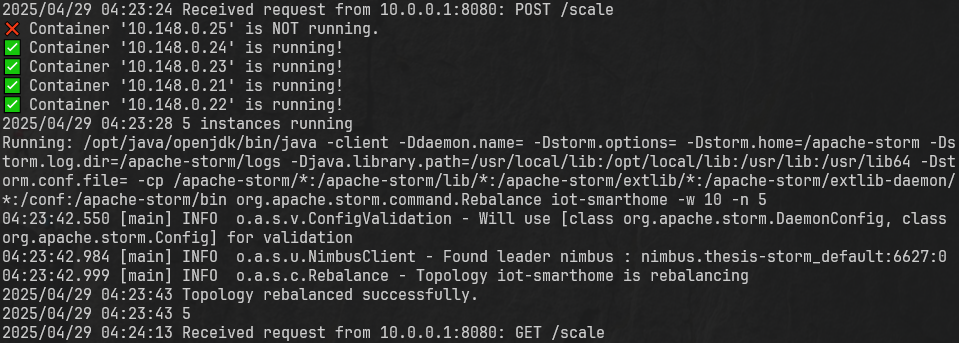
\includegraphics[width=\textwidth]{storm-autoscaler.png}
    \caption{Storm autoscaler}
\end{figure}

\subsection{Giai đoạn huấn luyện}

\begin{figure}[htbp]
    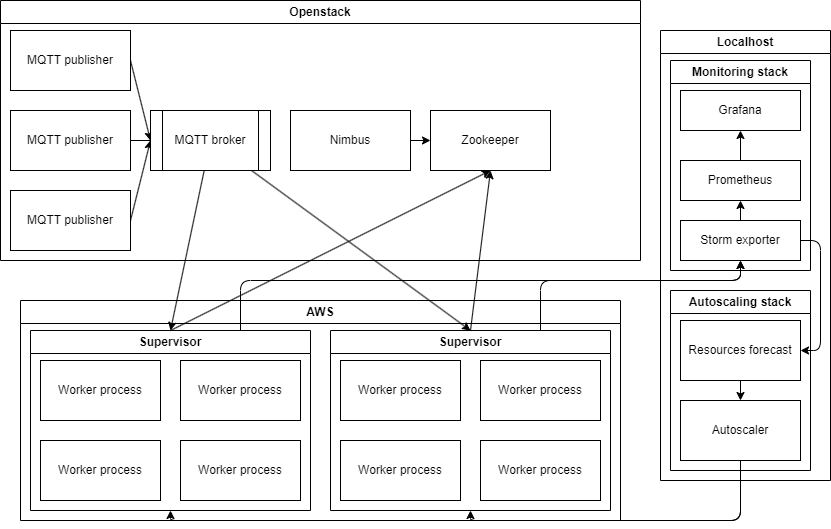
\includegraphics[width=\textwidth]{deployment.png}
    \caption{Sơ đồ triển khai hệ thống trong giai đoạn huấn luyện}
\end{figure}

Giai đoạn này có tác dụng xây dựng và tối ưu hóa bảng giá trị Q cho thuật toán học tăng cường, để hệ thống có thể tiếp xúc, tạo cơ sở về các đánh giá đối với môi trường được mô phỏng, giúp tăng hiệu quả và tốc độ trong giai đoạn sau, giai đoạn đánh giá.

\subsubsection{Triển khai cụm Apache Storm}

Các dịch vụ Nimbus, UI, Zookeeper, Supervisor được chạy trên máy chủ local bằng mô phỏng kiến trúc Docker Compose. Trong đó Storm Supervisor được chạy theo chế độ nhân bản với số lượng tối đa là năm và số lượng tối thiểu là hai. Cấu hình của mỗi Supervisor là 600 MB RAM và 1 vCPU.

\begin{lstlisting}[language=yaml, caption={Cấu hình của các supervisor}]
storm-supervisor:
    image: storm
    restart: always
    command: [storm, supervisor]
    volumes:
    - ./config/hosts:/etc/hosts:ro
    - ./config/storm.yml:/conf/storm.yaml
    deploy:
    replicas: 2
    resources:
        limits:
        memory: 600M
        cpus: 1
\end{lstlisting}

Do tất cả thành phần trên đều kết nối qua bridge network ảo của Docker được đảm bảo độ trễ giữa các dịch vụ không vượt quá 5ms - tương đương với độ trễ trong trung tâm dữ liệu. Mặc dù thành phần gửi dữ liệu (MQTT publisher) và các thành phần của cụm Storm đều nằm trên máy chủ nội bộ, giữa chúng còn có thành phần liên kết là MQTT broker được đặt tách biệt, vậy nên vẫn sẽ có độ trễ giống môi trường thật.Đây có thể coi như mô phỏng khá chính xác giữa môi trường trong giai đoạn huấn luyện với môi trường đánh giá hay thực tế sẽ được triển khai.

\subsubsection{Hệ thống co/dãn tài nguyên}

Docker Compose cung cấp cơ chế chạy các dịch vụ dưới dạng nhân bản (replicas). Dịch vụ trong Docker Compose là một tập các container. Đây sẽ là cơ sở để điều chỉnh số lượng supervisor trong môi trường huấn luyện. Người dùng có thể dễ dàng điều chỉnh số lượng nhân bản của một dịch vụ - cụ thể ở đây là storm-supervisor thông qua lệnh sau:

\begin{verbatim}
docker compose up -d --scale storm-supervisor <number_of_replicas>
\end{verbatim}

Quá trình huấn luyện sẽ được triển khai như đã trình bày tại chương trước, sau khi kết thúc toàn bộ ma trận Q được lưu vào tệp q\_table.npy.

\subsection{Giai đoạn đánh giá}

Giai đoạn này thử nghiệm mô hình trên môi trường điện toán đám mấy để kiểm tra hiệu năng thực tế, tính ổn định và khả năng thích ứng khi tải biến đổi.

\subsubsection{Triển khai máy ảo}

\begin{table}[h]
    \centering
    \resizebox{\textwidth}{!}{%
        \begin{tabular}{|l|l|l|l|l|l|l|}
            \hline
            Máy chủ           & Địa chỉ IP nội bộ    & \begin{tabular}[c]{@{}l@{}}Địa chỉ IP\\ công cộng\end{tabular} & Các dịch vụ chạy           & Cấu hình      & vCPU & \begin{tabular}[c]{@{}l@{}}RAM\\ (GB)\end{tabular} \\ \hline
            storm-manager     & 10.148.0.20          & Có                        & \begin{tabular}[c]{@{}l@{}}Storm Nimbus\\ Storm UI\\ Zookeeper\\ MySQL\\ Prometheus\\ Wireguard\\ Ansible\end{tabular} & e2-standard-2 & 2    & 8                         \\ \hline
            worker{[}0...4{]} & 10.148.0.{[}21-25{]} & Không                     & \begin{tabular}[c]{@{}l@{}}Supervisor\\ Container exporter\end{tabular} & e2-micro      & 2    & 1                         \\ \hline
            forecast          & Không                & Có                        & \begin{tabular}[c]{@{}l@{}}Storm forecast\\ Wireguard\end{tabular} & e2-micro      & 2    & 1                         \\ \hline
            publisher         & 10..148.0.11         & Không                     & MQTT publisher             & e2-micro      & 2    & 1                         \\ \hline
        \end{tabular}%
    }
    \caption{Bảng phân bố các dịch vụ trên các máy chủ GCP}
    \label{tab:gcp-services-distribution}
\end{table}

\begin{table}[h]
    \centering
    \resizebox{\textwidth}{!}{%
        \begin{tabular}{|l|l|l|l|l|}
            \hline
            Máy chủ        & Tên máy chủ   & Vị trí & Vai trò trong Wireguard & Địa chỉ IP Wireguard \\ \hline
            Storm manager  & storm-manager & GCP    & Server                  & 10.0.0.1             \\ \hline
            Storm forecast & forecast      & GCP    & Peer01                  & 10.0.0.2             \\ \hline
            Máy chủ cục bộ & localhost     & Cục bộ & Peer02                  & 10.0.0.3             \\ \hline
        \end{tabular}%
    }
    \caption{Phân bố vai trò và địa chỉ IP của các máy chủ trong VPN Wireguard}
    \label{tab:wireguard-distribution}
\end{table}

\begin{figure}[h]
    \centering
    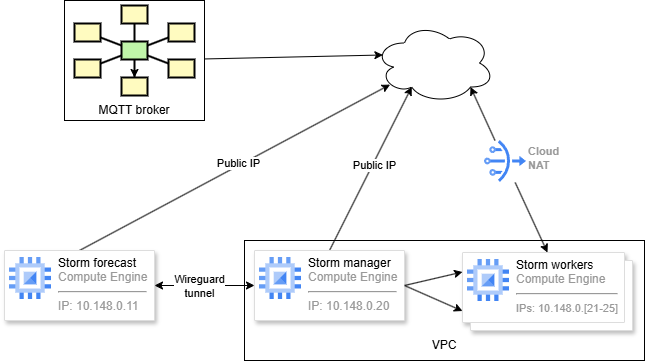
\includegraphics[width=\textwidth]{deployment-GCP.drawio.png}
    \caption{Sơ đồ triển khai GCP}
    \label{fig:deployment-gcp}
\end{figure}

\begin{figure}[h]
    \centering
    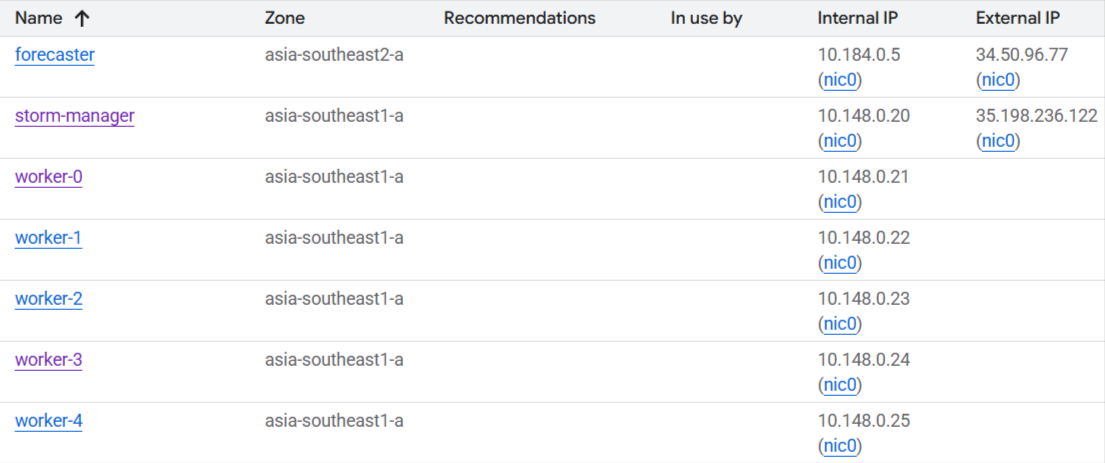
\includegraphics[width=\textwidth]{gcp-compute-engines.png}
    \caption{Khởi tạo máy ảo trên môi trường điện toán đám mây GCP}
\end{figure}

% Please add the following required packages to your document preamble:
% \usepackage{graphicx}
\begin{table}[h]
    \centering
    \resizebox{\textwidth}{!}{%
        \begin{tabular}{|l|l|l|l|l|l|}
            \hline
            Tên              & Nguồn                 & Hướng dữ liệu & Giao thức & Cổng                       & Đối tượng áp dụng          \\ \hline
            allow-ssh        & 0.0.0.0/0             & Vào/ra        & tcp       & 22                         & Tất cả                     \\ \hline
            allow\_wireguard & 0.0.0.0/0             & Vào           & udp       & 51820                      & Tất cả                     \\ \hline
            storm\_firewall  & Dải IP nội bộ của VPC & Vào/ra        & tcp       & \begin{tabular}[c]{@{}l@{}}6627\\ 6628\\ 8000\\ 2181\\ 6700\end{tabular} & \begin{tabular}[c]{@{}l@{}}storm-manager\\ worker-{[}0-4{]}\end{tabular} \\ \hline
            allow\_mysql     & Dải IP nội bộ của VPC & Vào           & tcp       & 3306                       & storm-manager              \\ \hline
        \end{tabular}%
    }
    \caption{Bảng danh sách các quy tắc tường lửa}
    \label{tab:firewall-rules}
\end{table}

Danh sách các máy chủ cùng với địa chỉ IP, cấu hình và các dịch vụ chúng chạy được liệt kê trong bảng \ref{tab:gcp-services-distribution}, sơ đồ thiết kế triển khai được minh họa trong hình \ref{fig:deployment-gcp}. Nhằm nâng cao tính bảo mật đồng thời đơn giản hóa việc áp dụng các quy tắc tường lửa, tác giả đã triển khai thêm hệ thống VPN WireGuard cho Storm manager, Storm forecast cùng với máy chủ cục bộ, cấu hình chi tiết được liệt kê trong bảng \ref{tab:wireguard-distribution}. Đối với các máy ảo trong cùng một VPC của GCP, cụ thể là Storm manager và các worker, việc triển khai WireGuard là không cần thiết do đã có hệ thống tường lửa có sẵn của GCP đồng thời các worker truy cập internet thông qua NAT router của GCP nên khả năng bị tấn công sẽ không có, do vậy ta chỉ cần mở các cổng tường lửa tương ứng với các cổng dịch vụ và thiết lập nguồn gửi trong cùng VPC là có thể đảm bảo hệ thống sẽ hoạt động chính xác. Danh sách các quy tắc tường lửa hệ thống áp dụng đã được liệt kê trong bảng \ref{tab:firewall-rules}.

Quá trình triển khai các máy ảo trên nền tảng GCP được tự động hóa thông qua công cụ Terraform, cho phép khởi tạo đồng thời nhiều máy ảo worker chạy Storm supervisor, dễ dàng điều chỉnh cấu hình và số lượng các worker. Mã nguồn quản lý toàn bộ kiến trúc hạ tầng của đồ án được tác giả viết và lưu trữ trong thư mục cloud của bộ mã nguồn của đồ án \autocite{lemionday_thesis_storm}.

Trong phạm vi luận án này, tác giả đã sử dụng 5 máy ảo worker. Các dịch vụ Storm supervisor được đóng gói và vận hành trong các container trên các máy ảo này, tạo điều kiện thuận lợi cho việc bật/tắt dịch vụ supervisor một cách linh hoạt. Về mặt chi phí, mô hình dự đoán tài nguyên cho phép tác giả cân nhắc việc sử dụng các máy ảo Spot VMs cho một số lượng worker nhất định, tận dụng dung lượng dư thừa của trung tâm dữ liệu trong thời gian thấp điểm để giảm chi phí vận hành máy ảo đến 91\%. Mặt khác, việc đặt chỗ trước (reserved instances) một số lượng máy ảo cũng là một giải pháp tiềm năng để tối ưu hóa chi phí, khi tài nguyên nhàn rỗi trong giai đoạn thấp điểm có thể được sử dụng cho các tác vụ tính toán khác, thay vì chỉ dành riêng cho hệ thống xử lý dữ liệu của ứng dụng SmartHome. Việc kết hợp các chiến lược này có tiềm năng giảm đáng kể tổng chi phí hệ thống.

\begin{lstlisting}[language=HCL, caption={Cấu hình khởi tạo máy ảo worker chạy Storm supervisor}]
resource "google_compute_instance" "worker" {
    count        = 5
    name         = "worker-${count.index}"
    machine_type = var.worker_machine_type
    zone         = var.zone

    boot_disk {
        initialize_params {
        image = "debian-cloud/debian-11"
        }
    }

    network_interface {
        network    = google_compute_network.storm_network.name
        network_ip = var.worker_internal_ips[count.index]
    }

    metadata_startup_script = join("\n",
        [
        file("./scripts/setup_docker.sh"),
        file("./scripts/setup_storm.sh"),
        file("./scripts/setup_storm_supervisor.sh"),
        file("./scripts/setup_docker_exporter.sh")
        ]
    )

    metadata = {
        ssh-keys = "storm:${file("./secrets/storm.pub")}"
    }

    tags = ["storm", "wireguard", "docker-access"]
}
\end{lstlisting}

\paragraph{Cấu hình Nimbus}

Do nền tảng Apache Storm không được thiết kế phù hợp đối với hệ thống co/dãn tài nguyên các supervisor, nguyên nhân là do cơ chế danh sách đen, trong khoảng thời gian dài nếu nimbus không nhận được phản hồi từ các supervisor, chúng sẽ bị đưa vào danh sách đen và phải sau một khoảng thời gian nhất định thì các supervisor này mới có thể được loại bỏ khỏi danh sách đen. Các supervisor ở trong danh sách đen sẽ không được phân phối công việc bởi nimbus, điều này ảnh hưởng rất lớn đến hoạt động của hệ thống khi chúng gây ra hai vấn đề. Vấn đề thứ nhất, số lượng các supervisor được phân phối công việc với số lượng supervisor trong tái cấu trúc (rebalance) không khớp nhau từ đó gây ra thiếu slot cần thiết để thực thi topology, thậm chí có thể khiến hệ thống ngừng xử lý dữ liệu. Vấn đề còn lại, do không được phân phối công việc, supervisor sẽ không có ý nghĩa trong topology, gây lãng phí tài nguyên. Vì lý do này thời gian để các supervisor được loại bỏ khỏi danh sách đen phải đủ ngắn để không bị đưa vào danh sách đen khi được bật trở lại sau khi tắt.

\begin{lstlisting}[language=yaml, caption={Cấu hình Nimbus node}]
storm.zookeeper.servers: [zookeeper]
nimbus.seeds: [nimbus]
ui.port: 8081

supervisor.slots.ports: [6700]

storm.blacklist.scheduler.tolerance.time.secs: 30
blacklist.scheduler.tolerance.time.secs: 30    # window to count failures
blacklist.scheduler.tolerance.count: 1        # failures to trigger exile
blacklist.scheduler.resume.time.secs: 30      # exile duration before return

storm.local.hostname: "nimbus.thesis-storm_default"
\end{lstlisting}

\paragraph{Triển khai ứng dụng xử lý dữ liệu SmartHome lên cụm Apache Storm}

Mã nguồn của topology sử dụng mã nguồn chương trình xử lý dữ liệu nhà thông minh xây dựng trên nền tảng Apache Storm \autocite{fimocodestormsmarthome} với một thay đổi nhỏ là MQTT broker được đổi thành broker.emqx.io. Đầu tiên ta tiến hành đẩy topology đã được biên dịch trên máy chủ cục bộ lên máy ảo storm-manager.

\begin{verbatim}
gcloud compute scp ./stormsmarthome/target/Storm-IOTdata-1.0-SNAPSHOT-jar-with-dependencies.jar storm@storm-manager:~/thesis-storm/stormsmarthome/target   
\end{verbatim}

Sau đó tiến hành triển khai topology tại container nimbus.

\begin{verbatim}
docker exec nimbus storm jar /topologies/Storm-IOTdata-1.0-SNAPSHOT-jar-with-dependencies.jar com.storm.iotdata.MainTopo
\end{verbatim}


\paragraph{Máy ảo supervisor}

Trên mỗi máy ảo supervisor sẽ triển khai hai dịch vụ chính: Container exporter \autocite{shayan_ghani_containerexporter} và Storm supervisor. Trong đó, Container exporter đảm nhiệm việc cung cấp các thông số giám sát hệ thống thông qua đường dẫn \textit{/metrics}, mặc định được lắng nghe tại cổng \textit{8000}. Khác với giai đoạn huấn luyện, khi Storm exporter trực tiếp thu thập dữ liệu từ Docker API của các supervisor cục bộ, trong môi trường triển khai thực tế, nó sẽ thu thập dữ liệu từ đường dẫn \textit{/metrics} của các máy ảo worker. Sau đó, Storm exporter tổng hợp, chuyển đổi tên các metric và bổ sung nhãn để đảm bảo tính thống nhất giữa các môi trường với các truy vấn dữ liệu của hệ thống Storm forecast.

\begin{lstlisting}[language=yaml, caption={Cấu hình các dịch vụ chạy trên máy ảo supervisor}]
services:
    cxp:
        image: devopsteen/cxp:latest
        container_name: container-exporter
        volumes: [/var/run/docker.sock:/var/run/docker.sock]
        ports: [8000:8000]
        environment:
            CONTAINER_EXPORTER_PORT: ${CONTAINER_EXPORTER_PORT}
        restart: always

    storm-supervisor:
        image: storm
        restart: always
        command: [storm, supervisor]
        network_mode: host
        volumes:
        - ./config/hosts.cloud:/etc/hosts:ro
        - ./config/storm.cloud.yml:/conf/storm.yaml
        deploy:
        resources:
            limits:
            memory: 600M
            cpus: 1
\end{lstlisting}

Mỗi supervisor chỉ sử dụng một port duy nhất cho chúng chỉ được cấp 1 CPU, giới hạn bộ nhớ và cpu lần lượt là 600Mb và 100 - tương ứng với 1 CPU.
\begin{lstlisting}[language=yaml, caption={Cấu hình của dịch vụ supervisor}]
storm.zookeeper.servers: [10.148.0.20]
nimbus.seeds: [nimbus.thesis-storm_default]

supervisor.slots.ports:
- 6700

supervisor.memory.capacity.mb: 600
supervisor.cpu.capacity: 100
\end{lstlisting}

\subsection{Triển khai chương trình dự đoán số lượng supervisor - Storm forecast}

Mã nguồn chương trình được tác giả đồ án viết và lưu tại thư mục forecast trong bộ mã nguồn của đồ án \autocite{lemionday_thesis_storm}.

Trong môi trường huấn luyện, lệnh chạy là

\begin{verbatim}
python3 q_learning_agent.py 
\end{verbatim}

Đường dẫn mặc định đến Prometheus là \href{http://localhost:9090}{http://localhost:9090} và đến chương trình autoscaler là \href{http://localhost:8083}{http://localhost:8083}.

Trong môi trường đánh giá, máy ảo storm-manager sẽ chạy dịch vụ wireguard server giúp việc truy cập các dịch vụ trên máy ảo này từ localhost dễ dàng và bảo mật, mặc định địa chỉ của wg0 được gán là 10.0.0.1. Lệnh chạy là

\begin{verbatim}
PROMETHEUS_URL=http://10.0.0.1:9090 \\
AUTOSCALER_URL=http://10.0.0.1:8080 \\
python3 q_learning_agent.py
\end{verbatim}

\begin{figure}[H]
    \centering
    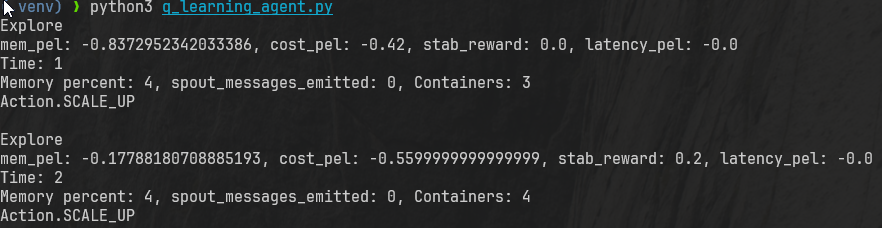
\includegraphics[width=\textwidth]{training-start.png}
    \caption{Bắt đầu quá trình huấn luyện}
\end{figure}

\begin{figure}[H]
    \centering
    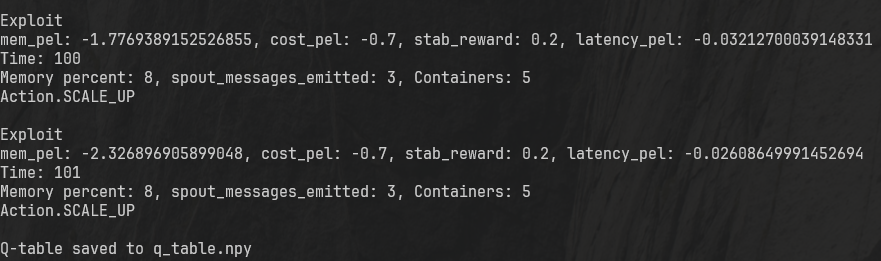
\includegraphics[width=\textwidth]{training-save-q-table.png}
    \caption{Lưu bảng giá trị Q sau khi huấn luyện}
\end{figure}
% \includegraphics[width=0.5\textwidth]{deployment.svg}

% \section{Hệ thống Storm SmartHome}

% \subsection{Hệ thống xử lý dữ liệu lên GCP}
% Hệ thống xử lý dữ liệu bao gồm 4 máy ảo (1 core, 1vCPU) chạy dịch vụ Storm supervisor. Để đơn giản hóa việc triển khai, ta có thể coi việc bật/tắt các dịch vụ Storm supervisor tương đương với việc thêm/xóa các máy ảo chạy dịch vụ Storm supervisor.
% Trên các máy ảo này sẽ được cài thêm chương trình \autocite{prometheus_node_exporter} để thu thập các thông số của máy ảo nhằm cung cấp cho prometheus để đánh giá hiệu năng hệ thống và storm-forecast để dự đoán hệ thống.

% \subsection{Hệ thống theo dõi số liệu}

% \subsubsection{Storm exporter}

% Chương trình lấy từ storm topology các thông số về spout, bolt, topology.

% \subsubsection{Prometheus}

% Thu thập dữ liệu từ storm-exporter, thông số hiệu năng của storm supervisor

% \subsubsection{Grafana}

% Đồ thị hóa các thông số Prometheus thu thập được.

% \subsection{Hệ thống dự đoán tài nguyên}

% \subsubsection{Giai đoạn đào tạo}
% Trong giai đoạn này, chương trình dự đoán tài nguyên được chạy nhiều lần với các thông số đầu vào là thông số hiệu năng của các Storm supervisor, latency trung bình của topology, spout throughput của hệ thống mạng. Từ các thông số đầu vào, tiến hành dự đoán số lượng máy ảo cần sử dụng trong tương lai, dự đoán này được gửi cho chương trình strom-autoscaler để tiến hành điều chỉnh tài nguyên. Sau khi điều chỉnh tài nguyên và tiến hành tái cân bằng (rebalance) hệ thống mạng, các thông số đầu vào được cập nhật để tiến hành đánh giá hiệu quả. Quá trình lặp lại nhiều lần, mỗi lần trong thời gian 10s để tiến đến mô hình huấn luyện tối ưu. Sau khi kết thúc quá trình huấn luyện, mô hình đã được huấn luyện sẽ được lưu lại và sử dụng trong giai đoạn đánh giá. Mục tiêu của dự đoán là giữ spout throughput, latency của topology, cpu và memory usage của máy ảo ở trong ngưỡng bình thường nhưng đồng thời sử dụng số lượng máy ảo là ít nhất.

% \subsubsection{Giai đoạn đánh giá}
% Trong giai đoạn này, dựa trên mô hình đã được huấn luyện, ta tiến hành chạy và đánh giá hiệu quả của chương trình với môi trường của các Storm supervisor là máy ảo trong môi trường AWS.

% \subsection{Hệ thống co dãn Storm-autoscaler}

% \subsubsection{Giai đoạn đào tạo}
% Hệ thống là các máy ảo trong môi trường Openstack

% \subsubsection{Giai đoạn đánh giá}
% Hệ thống là các máy ảo trong môi trường AWS


% \section{Triển khai hệ thống}
% Phần triển khai bao gồm hai giai đoạn chính: \textbf{huấn luyện} và \textbf{đánh giá—triển khai thực tế}. Mỗi giai đoạn được mô tả chi tiết dưới đây.

% \subsection{Giai đoạn huấn luyện (Local)}
% \label{sec:training-local}

% \subsubsection{Mục tiêu và kiến trúc tổng quát}
% Giai đoạn huấn luyện nhằm xây dựng và tối ưu hóa bảng Q (Q-table) cho thuật toán học tăng cường, từ đó hệ thống có khả năng học cách co giãn đa cấp độ chủ động. Mô hình gồm:
% \begin{itemize}
%     \item \textbf{MQTT Broker} và \textbf{MQTT Publisher:}
%           \begin{itemize}
%               \item Broker chạy trên nền OpenStack, không giới hạn băng thông.
%               \item Publisher mô phỏng dữ liệu tải từ 3 tòa nhà (building A, B, C), mỗi tòa nhà phát luồng dữ liệu telemetry về trạng thái CPU, RAM, độ trễ mạng, v.v.
%           \end{itemize}
%     \item \textbf{Apache Storm Cluster:}
%           \begin{itemize}
%               \item \emph{Nimbus}, \emph{UI}, \emph{Zookeeper} khởi động trên máy chủ local.
%               \item 5 node \emph{Supervisor} chạy trên cùng host, mỗi node cấu hình: 700 MB RAM, 1 vCPU.
%               \item Số lượng worker slot động: tối thiểu 2, tối đa 5.
%           \end{itemize}
% \end{itemize}

% \subsubsection{Cấu hình phần cứng và mạng}
% \begin{itemize}
%     \item Tất cả thành phần Local kết nối qua bridge network ảo Docker.
%     \item MQTT Broker và Publisher chạy trên network \texttt{openstack-net}, Storm cluster trên \texttt{local-net}.
%     \item Đảm bảo latency nội bộ dưới 5 ms để phản ánh môi trường trung tâm dữ liệu thực.
% \end{itemize}

% \subsubsection{Chi tiết huấn luyện Reinforcement Learning}
% \paragraph{Đặc tả Môi trường (Environment)}
% \begin{itemize}
%     \item \emph{State} bao gồm: số lượng worker hiện tại, CPU utilization trung bình, queue depth, throughput.
%     \item \emph{Action} là tăng hoặc giảm số worker (±1) trong khoảng [2, 5].
%     \item \emph{Reward} tính theo hàm:
%           \[
%               r = -\alpha \times \text{CPU\_util\%} - \beta \times \text{latency} + \gamma \times \text{throughput},
%           \]
%           với $\alpha, \beta, \gamma$ cân chỉnh để ưu tiên độ trễ thấp và hiệu năng cao \cite{qlearning1967}.
% \end{itemize}

% \paragraph{Thuật toán và siêu tham số}
% \begin{itemize}
%     \item Sử dụng Q-learning $\epsilon$-greedy:
%           \[
%               Q(s,a) \leftarrow Q(s,a) + \eta \bigl(r + \gamma \max_{a'} Q(s',a') - Q(s,a)\bigr).
%           \]
%     \item Hệ số học (learning rate) $\eta = 0.1$, hệ số khấu hao (discount factor) $\gamma = 0.99$.
%     \item Epsilon khởi tạo $\epsilon = 1.0$, giảm dần đến $\epsilon_{min} = 0.05$ trong suốt 10\,000 bước \cite{rlSurvey2020}.
%     \item Số tập huấn luyện (episodes): 5\,000, mỗi episode gồm 100 bước tương tác.
% \end{itemize}

% \paragraph{Quy trình huấn luyện}
% \begin{enumerate}
%     \item Khởi tạo Storm cluster và MQTT môi trường mô phỏng.
%     \item Chạy vòng lặp chính trong một goroutine hoặc thread Python:
%           \begin{itemize}
%               \item Đọc state mới từ bolt xử lý message MQTT.
%               \item Lựa chọn action theo chính sách $\epsilon$-greedy.
%               \item Gửi command thay đổi worker thông qua REST API của Storm.
%               \item Nhận reward và state kế tiếp.
%               \item Cập nhật Q-table.
%           \end{itemize}
%     \item Mỗi 100 episode, lưu checkpoint Q-table xuống local.
%     \item Kết thúc huấn luyện, toàn bộ ma trận Q được lưu vào file \texttt{q\_table.npy}.
% \end{enumerate}

% \subsection{Giai đoạn đánh giá và triển khai (GCP)}
% \label{sec:deployment-gcp}

% \subsubsection{Mục tiêu và tổng quan}
% Chuyển mô hình đã huấn luyện lên môi trường Cloud để kiểm chứng hiệu năng thực tế, tính ổn định và khả năng thích ứng nhanh với biến đổi tải.

% \subsubsection{Mô hình hạ tầng trên GCP}
% \begin{description}
%     \item[Storm Manager VM (e2‑standard‑2):]
%           \begin{itemize}
%               \item Chạy các dịch vụ: Nimbus, Zookeeper, Storm UI, MySQL (lưu lịch sử scale).
%               \item Triển khai \emph{WireGuard Server} để mã hóa và bảo mật liên kết giữa các VM \cite{wireguard2017}.
%               \item Gán \emph{public IP} tĩnh để truy cập UI và quản trị.
%           \end{itemize}

%     \item[Supervisor Nodes (5 × e2‑micro):]
%           \begin{itemize}
%               \item Chạy Storm Supervisor và \texttt{container\_exporter} để thu thập metrics CPU, RAM, I/O \cite{container_exporter2018}.
%               \item Dịch vụ Supervisor được bật/tắt tự động tương ứng với lệnh scale VM.
%               \item Mỗi node có \emph{static internal IP} trong VPC để Storm Manager kết nối ổn định.
%           \end{itemize}

%     \item[MQTT Publisher VM (e2‑micro):]
%           \begin{itemize}
%               \item Chạy script Python mô phỏng 3 tòa nhà, publish lên broker công cộng \texttt{broker.emqx.io} \cite{emqx2021}.
%               \item VM này được gán static internal IP và kết nối ra Internet.
%           \end{itemize}

%     \item[Forecast VM (e2‑micro):]
%           \begin{itemize}
%               \item Chạy WireGuard Client để truy cập private network của Storm Manager.
%               \item Gán public IP để dễ điều khiển và tinh chỉnh tham số trong thời gian chạy.
%           \end{itemize}
% \end{description}

% \subsubsection{Kết nối và bảo mật}
% \begin{itemize}
%     \item Thiết lập VPC riêng, subnet cho Storm và subnet cho MQTT Publisher/Forecast.
%     \item WireGuard kết nối point-to-site từ Forecast và Publisher đến Storm Manager.
%     \item Firewall rules hạn chế chỉ mở port 6627 (Storm Thrift), 8080 (UI), 2181 (Zookeeper), 51820 (WireGuard).
% \end{itemize}

% \subsubsection{Triển khai Q-table và chính sách epsilon}
% \begin{itemize}
%     \item File \texttt{q\_table.npy} được upload lên Storm Manager, bolt khởi động tải vào memory.
%     \item Thiết lập $\epsilon = \epsilon_{min} = 0.05$ để giữ khả năng khám phá nhẹ nhàng trong thực tế, thích ứng với thay đổi về mô tả tải.
% \end{itemize}

% \subsection{Đánh giá hiệu năng và thu thập dữ liệu}
% \label{sec:evaluation}
% \begin{itemize}
%     \item \textbf{Chỉ số đo lường:}
%           \begin{itemize}
%               \item \emph{Response time} trung bình và P95 của hệ thống xử lý dữ liệu.
%               \item \emph{Resource utilization} (CPU, RAM) trên Supervisor nodes.
%               \item \emph{Scale event count}: số lần scale up/down trên mỗi khoảng thời gian.
%           \end{itemize}
%     \item \textbf{Công cụ thu thập:}
%           \begin{itemize}
%               \item Prometheus + Grafana kết hợp với \texttt{container\_exporter} để giám sát real-time.
%               \item Storm UI logs để xác nhận trạng thái topology.
%               \item MySQL lưu lịch sử scale để phân tích bằng Python.
%           \end{itemize}
%     \item \textbf{Quy trình đánh giá:}
%           \begin{enumerate}
%               \item Kích hoạt tải mô phỏng tăng giảm theo kịch bản (peak, off-peak).
%               \item Ghi nhận chỉ số trong 2 giờ liên tục.
%               \item So sánh với baseline (auto-scaling căn bản dựa trên ngưỡng CPU).
%               \item Phân tích kết quả: ưu nhược điểm, thời gian hội tụ, tần suất scale.
%           \end{enumerate}
% \end{itemize}